\section{Introduction}\label{sec:introduction}

This paper is an extended version of a VLDB 2023
publication~\cite{budiu-vldb23}, adopting the notations
from~\cite{budiu-sigmod24}.  The major changes are: adding new
incremental program examples (\refsec{sec:recursive-example},
\refsec{sec:recursive-incremental-example}), an expanded
implementation section~\refsec{sec:implementation}, and an
experimental evaluation~\refsec{sec:experiments}.  This paper includes
only a few short mathematical proofs; all the proofs can be found in
an extended technical report~\cite{tr}; the proofs have also been
formalized and verified in the Lean proof
assistant~\cite{dbsp-theory}.

\subsection{Problem and Solution Overview}\label{sec:intro-incremental}

The IVM problem can be stated as follows: we are given a database $DB$
and a view $V$, described by a query $Q$.  The goal of IVM is to keep
the contents of $V$ up-to-date in response to changes of the database.

Consider the following SQL statement:

\begin{lstlisting}[language=SQL]
CREATE VIEW V AS
SELECT * FROM T WHERE Age >= 10
\end{lstlisting}

In this example the query $Q$ defining the view $V$ is the
\code{SELECT} statement.  The view \code{V} always contains all the
rows of table \code{T} whose value for the column \code{Age} is
greater than or equal to 10.

In general a query is a function applied to the contents of a
database: $V = Q(DB)$.  A na\"ive solution re-executes query $Q$ every
time the database changes, as illustrated in the following diagram.
Time is the horizontal axis; the horizontal arrows labeled with
$\Delta$ depict changes to the database.  The ``up'' arrows show the
re-evaluation of $Q$ for each database snapshot.

\noindent 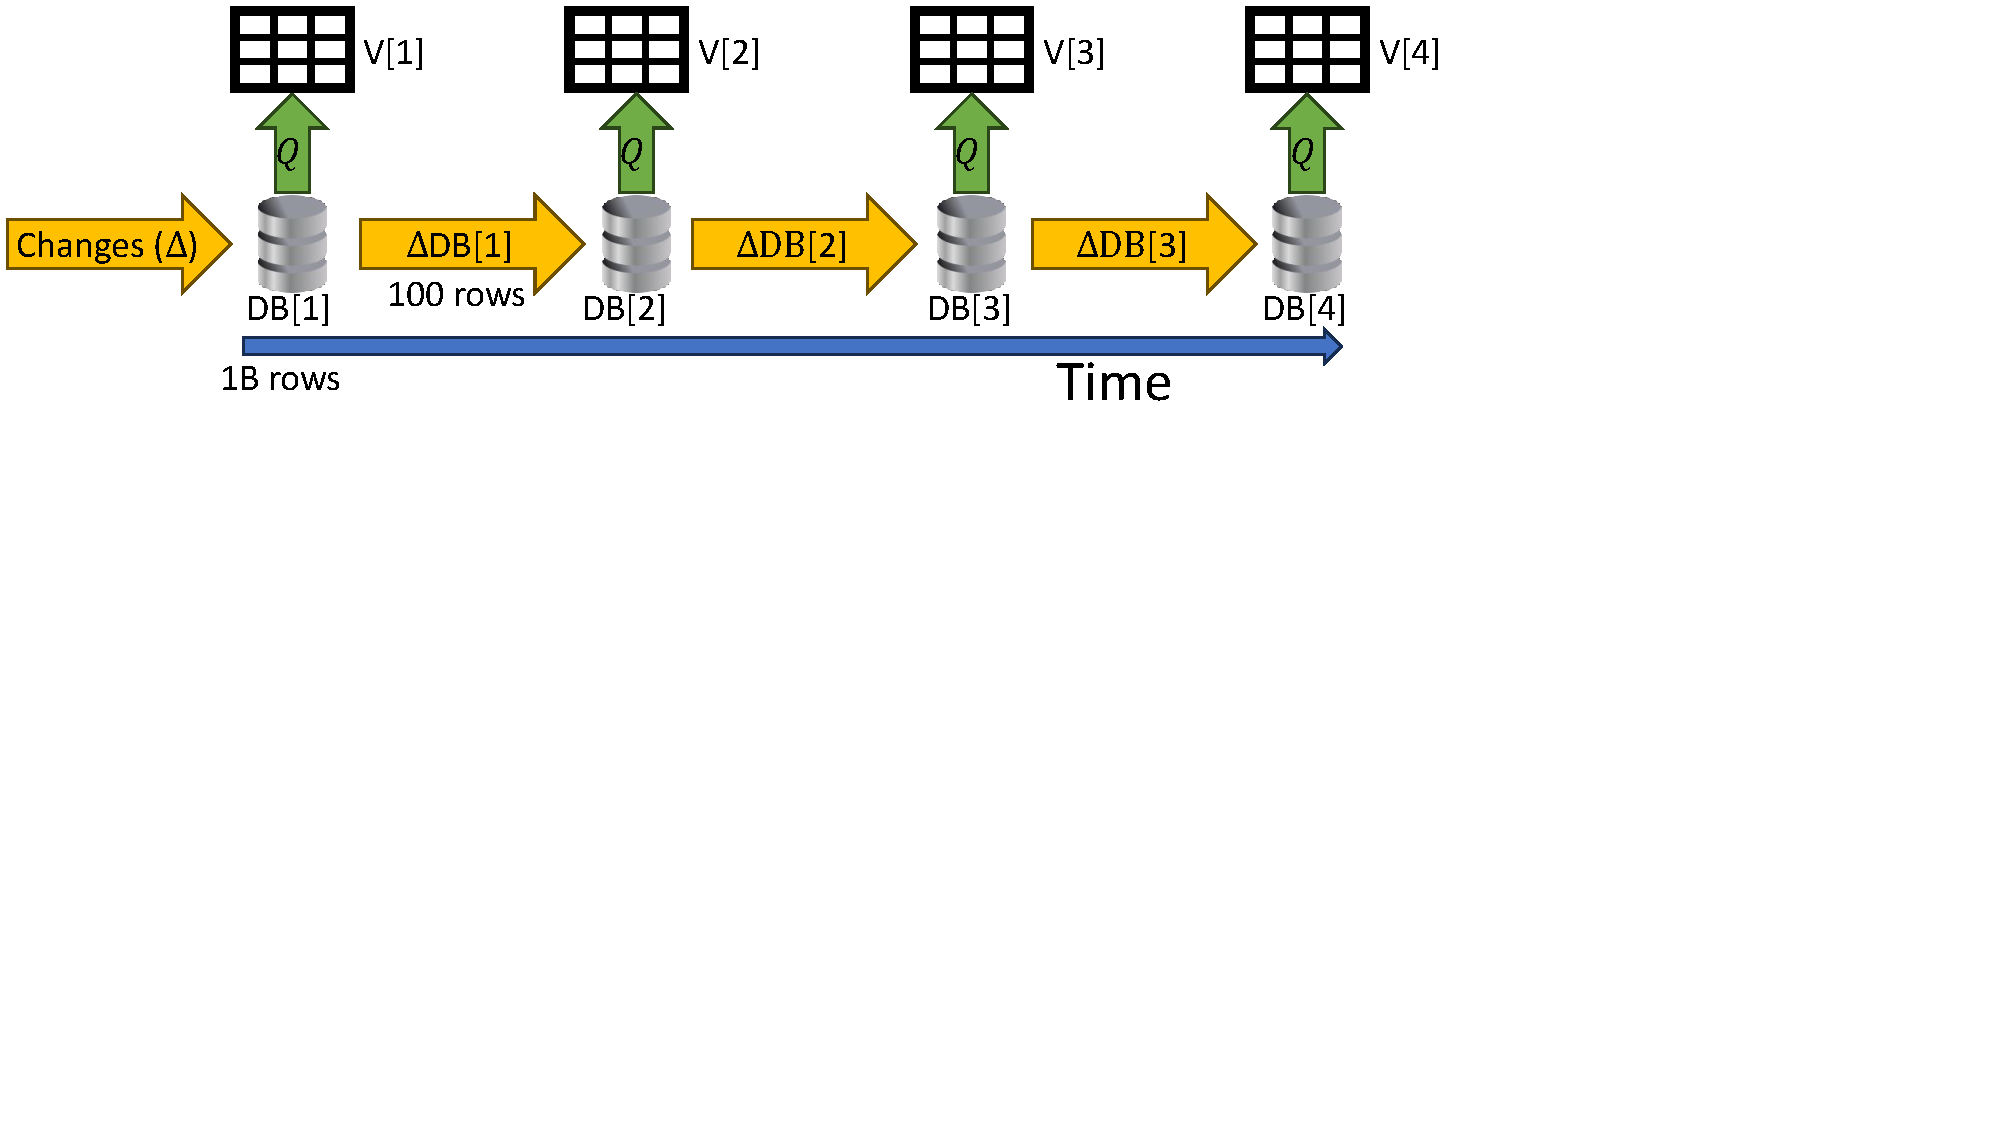
\includegraphics[trim={0 4.8in 3.7in 0},clip,scale=.34]{view.pdf}

The naive solution is expensive.  After the first version of the view
has been constructed, an ideal algorithm would compute only
\emph{changes} to the view $\Delta V$ doing work $O(|\Delta DB|)$.
Ideally, we want to construct a new query $\inc{Q}$ with the property
that $\Delta V = \inc{Q}(\Delta DB)$, i.e., $\inc{Q}$ can compute the
change of the view from the change of the database:

\noindent 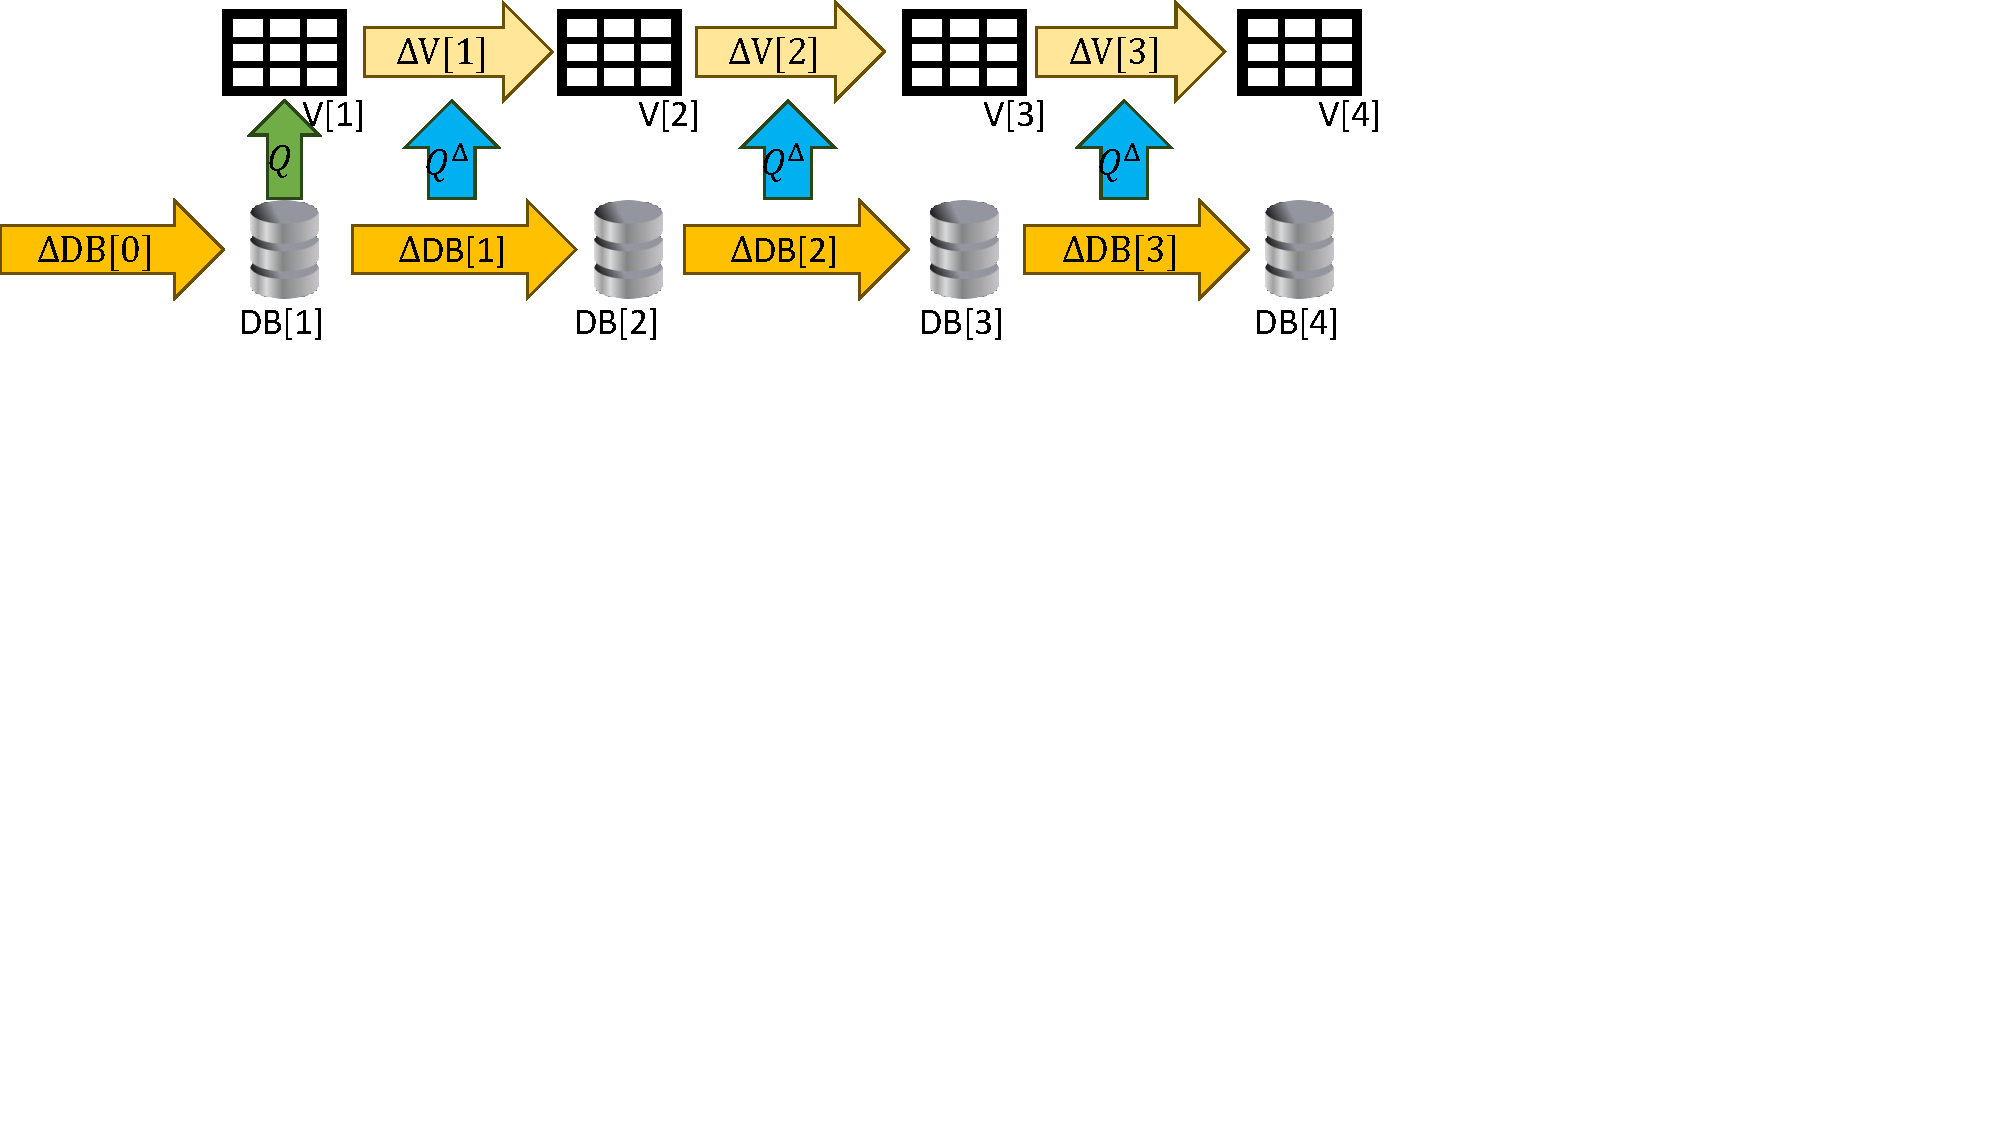
\includegraphics[trim={0 5.2in 4.1in 0},clip,scale=.35]{incview.pdf}

We call $\inc{Q}$ the \emph{incremental} version of $Q$.  If we want
$\inc{Q}$ to be a function of $\Delta DB$, one can show that the ideal
solution as described above is impossible to reach.

In this paper we propose a new way to define $\inc{Q}$, as a form of
\emph{computation on streams}.  Our model is inspired by Digital
Signal Processing DSP~\cite{rabiner-book75}, applied to databases,
hence the name \dbsp.

$\inc{Q}$ can be significantly more efficient than the na\"ive
solution.  As is the case for traditional database queries, the
performance of $\inc{Q}$ depends both on the query $Q$ but also on the
actual data that the query is applied to.  Informally, $\inc{Q}$ built
by our algorithm, is faster than $Q$ by a factor of $O(|DB| / |\Delta
DB|)$.  In practice this may be an improvement of several orders of
magnitude.

Instead of treating the database as a large, changing object, we model
it as a sequence or \emph{stream} of database snapshots, shown as
$DB[1], DB[2], \ldots$ previously.  Similarly, consecutive view
snapshots form a stream.  \dbsp is a simple programming language
computing on streams; inputs and outputs are streams of arbitrary
values.

The \dbsp language has only 4 operators.  However, it can express a
rich set of computations on streams, including repeated computations
(similar to the repeated queries $Q$ above), recursive computations
that compute fixed points (like Datalog programs), more general
streaming computations, and incremental computations (defined
shortly).

The central result of this paper is Algorithm~\ref{algorithm-inc}
in~\refsec{sec:relational}.  The input to the algorithm is a \dbsp
program that computes on a stream of data; the algorithm mechanically
transforms it into an incremental \dbsp program that computes on a
stream of changes.

\dbsp is not tied to databases in any way; it is in fact a
Turing-complete language that can be used for many other purposes.
But it works particularly well in the area of databases, for two
reasons:

\begin{itemize}[nosep, leftmargin=0pt, itemindent=0.5cm]
  \item \dbsp operates on values from a commutative group.  Databases
    can be modeled as a commutative group.
  \item \dbsp reduces the problem of incrementalizing a complex
    program to the problem of incrementalizing each primitive
    operation that appears in the program.  For databases there are
    known efficient incremental implementations for all primitive
    operations.
\end{itemize}

\subsection{Core abstractions}

\subsubsection{Circuits}

In this paper we use circuit diagrams to depict programs.  In a
circuit a rectangle represents a function, and an arrow represents an
input or output value.  The following diagram shows a function $f$
consuming two inputs $i$ (input 0) and $j$ (input 1) and producing one
output $o = f(i, j)$:
%
\begin{center}
\begin{tikzpicture}[auto,>=latex,inner sep=0mm]
  \node[block, minimum height=.6cm, minimum width=.5cm] (function) {$f$};
  \node[below=1mm of function.north west,font=\tiny,anchor=north west] (0) {0};
  \node[above=1mm of function.south west,font=\tiny,anchor=south west] (1) {1};
  \node[left of=0, node distance=.5cm] (input0) {$i$};
  \node[left of=1, node distance=.5cm] (input1) {$j$};
  \node[right of=function, node distance=.8cm] (output) {$o$};
  \draw[->] (input0) -- (0);
  \draw[->] (input1) -- (1);
  \draw[->] (function) -- (output);
\end{tikzpicture}
\end{center}

%
Most of the functions we deal with are commutative, so we omit input
labels, showing the circuit above as:
%
\begin{center}
  \begin{tikzpicture}[auto,>=latex, node distance=.7cm]
    \node[] (input0) {$i$};
    \node[below of=input0,node distance=.15cm] (dummy) {};
    \node[below of=dummy,node distance=.15cm] (input1) {$j$};
    \node[block, right of=dummy] (T) {$f$};
    \node[right of=T] (output) {$s$};
    \draw[->] (input0) -- (T);
    \draw[->] (input1) -- (T);
    \draw[->] (T) -- (output);
  \end{tikzpicture}
\end{center}

%
Functions, and their circuits, can be composed, as in the following
example showing $o = g(s) + (f(s) \times s)$:
%
\begin{center}
\begin{tikzpicture}[auto,>=latex]
  \node[] (input) {$s$};
  \node[] [right of=input, node distance=.4cm] (dummy) {};
  \node[block, below of=dummy, node distance=.65cm] (S1) {$f$};
  \node[block, right of=S1] (T1) {$\times$};
  \node[block, right of=T1] (T2) {$+$};
  \node[block, above of=T2, node distance=.65cm] (S2) {$g$};
  \node[right of=T2, node distance=.7cm] (output) {$o$};
  \draw[->] (input) -| (S1);
  \draw[->] (input) -| (T1);
  \draw[->] (S1) -- (T1);
  \draw[->] (T1) -- (T2);
  \draw[->] (input) -- (S2);
  \draw[->] (T2) -- (output);
  \draw[->] (S2) -- (T2);
\end{tikzpicture}
\end{center}

\subsubsection{Streams}

The core notion of \dbsp is the \textbf{stream}.  Given a set $A$, a
\defined{stream} \emph{of values from $A$} is an infinite sequence of
values from $A$.  $\stream{A}$ denotes the set of all streams with
values from $A$.  We write $s[t]$ for the $t$-th element of the stream
$s$.  Think of $t$ as the ``time'' and of $s[t]\in A$ as the value of
the stream $s$ ``at time'' $t$.  We show streams as a sequence of
boxes, with time from \emph{right to left}: e.g., the stream $id[t]
\defn t$ is:
%
\begin{center}
\begin{tabular}{cc}
  \sv{0 1 2 3 4} \\
  $\xleftarrow[\hspace{1cm}\mathrm{time}\hspace{1cm}]{}$
\end{tabular}
\end{center}

A \defined{stream operator} is a function that computes on streams and
produces streams.  We use ``operator'' for streams, and ``function''
for computations on ``scalar'' values.  In circuits we use arrows with
a double head to depict streams.  The following diagram shows a stream
operator $T$ consuming two input streams $s_0$ and $s_1$, producing
one output stream $s$; the difference from the previous figure is in
the use of double arrows.
%
\begin{center}
\begin{tikzpicture}[auto,>=latex,inner sep=0mm]
  \node[block, minimum height=.6cm, minimum width=.5cm] (function) {$T$};
  \node[below=1mm of function.north west,font=\tiny,anchor=north west] (0) {0};
  \node[above=1mm of function.south west,font=\tiny,anchor=south west] (1) {1};
  \node[left of=0, node distance=0.8cm] (input0) {$s_0$};
  \node[left of=1, node distance=0.8cm] (input1) {$s_1$};
  \node[right of=function, node distance=.8cm] (output) {$s$};
  \draw[->>] (input0) -- (0);
  \draw[->>] (input1) -- (1);
  \draw[->>] (function) -- (output);
\end{tikzpicture}
\end{center}
%
We write $s = T(s_0, s_1)$.
%\begin{definition}(lifting)
Given a function $f: A \to B$, we define a stream operator $\lift{f}
:\stream{A} \to \stream{B}$ (read as ``$f$ lifted'') by applying
function $f$ to each input value independently:

\noindent
\begin{center}
  \begin{tikzpicture}[auto,>=latex]
    \node[] (input) {$\sv{a b c d e}$};
    \node[block, right of=input, node distance=2cm] (f) {$\lift{f}$};
    \node[right of=f, node distance=2.6cm] (output) {$\sv{f(a) f(b) f(c) f(d) f(e)}$};
    \draw[->>] (input) -- (f);
    \draw[->>] (f) -- (output);
  \end{tikzpicture}
\end{center}
%\end{definition}

\subsection{Databases as streams}

We generally think of streams as sequences of ``small'' values, such
as insertions or deletions in a database.  However, we also treat the
whole database as a \emph{stream of database snapshots}.  We model a
database as a stream $DB$.  Time is not wall-clock time, but counts
the transactions executed.  Since transactions are linearizable, they
have a total order.  $DB[t]$ is the snapshot of the database contents
after $t$ transactions have been applied.  We use this notation in the
diagrams in \refsec{sec:intro-incremental}.

Database transactions also form a stream $\Delta DB$, this time a
stream of \emph{changes}, or \emph{deltas}, that are applied to the
database.  The values of this stream are defined by $(\Delta DB)[t] =
DB[t] - DB[t-1]$, where ``$-$'' stands for the difference between two
databases, a notion that we will soon make more precise.  The $\Delta
DB$ stream can be produced from the $DB$ stream by the \emph{stream
differentiation} operator $\D$; this operator produces as its output
the stream of changes from its input stream; we have thus $\D(DB) =
\Delta DB$.

Conversely, the database snapshot at time $t$ is the cumulative result
of applying all transactions up to $t$: $DB[t] = \Delta DB[0] + \Delta
DB[1] + \ldots + \Delta DB[t]$.  The stream operator $\I$ is defined
to produce each output by adding up all previous inputs.  We call $\I$
\emph{stream integration}, the inverse of differentiation.  The
following diagram shows the relationship between the streams $\Delta
DB$ and $DB$:
\begin{center}
\begin{tikzpicture}[auto,>=latex,minimum width=.5cm, node distance=1.2cm]
  \node[] (input) {$\Delta DB$};
  \node[block, right of=input] (I) {$\I$};
  \node[right of=I] (output) {$DB$};
  \node[block, right of=output] (D) {$\D$};
  \node[right of=D] (end) {$\Delta DB$};
  \draw[->>] (input) -- (I);
  \draw[->>] (I) -- (output);
  \draw[->>] (output) -- (D);
  \draw[->>] (D) -- (end);
\end{tikzpicture}
\end{center}

In this model a database view is also a stream.  Suppose query $Q$
defining a view $V$.  For each snapshot of the database stream we have
a snapshot of the view: $V[t] = Q(DB[t])$.  A view is thus just a
lifted query: $V = (\lift{Q})(DB)$.

Armed with these basic definitions, we can precisely define IVM.  A
maintenance algorithm computes the \emph{changes} to the view given
the changes to the database. Given a query $Q$, a key contribution of
this paper is the definition of its \emph{incremental version}
$\inc{Q}$, using stream integration and differentiation, depicted
graphically as:

%
\begin{center}
\begin{tikzpicture}[auto,>=latex,minimum width=.5cm]
  \node[] (input) {$\Delta DB$};
  \node[block, right of=input, node distance=1.3cm] (I) {$\I$};
  \node[block, right of=I, node distance=1.3cm] (Q) {$\lift{Q}$};
  \node[block, right of=Q, node distance=1.3cm] (D) {$\D$};
  \node[right of=D] (output) {$\Delta V$};
  \draw[->>] (input) -- (I);
  \draw[->>] (I) -- node (db) {$DB$} (Q);
  \draw[->>] (Q) -- node (B) {$V$} (D);
  \draw[->>] (D) -- (output);
  \draw[decorate, decoration = {brace, raise=12pt}] (input) -- (output)
  node[pos=.5, above=12pt]{$\inc{Q}$};
\end{tikzpicture}
\end{center}

%
Mathematically: $\inc{Q} = \D \circ (\lift{Q}) \circ \I$.  The
incremental version of a query $Q$ is a \emph{streaming operator}
$\inc{Q}$ which computes directly on changes and produces changes.
The incremental version of a query is thus always well-defined.  The
above definition gives us one way to compute a query incrementally,
but applying it naively produces an inefficient execution, since it
reconstructs the database at each step.  It is in fact as bad as the
naive solution.  In \refsec{sec:incremental} we show how we can
optimize the implementation of $\inc{Q}$. The key property is that the
we can ``push'' the $\inc{.}$ operator ``down'' in a query plan:
$\inc{(Q_1 \circ Q_2)} = \inc{Q_1} \circ \inc{Q_2}$.

Armed with this general theory of incremental computation, in
\secref{sec:relational} we show how to model relational queries in
\dbsp.  This immediately gives us a general algorithm to compute the
incremental version of any relational query.  These results were
previously known, but they are cleanly modeled by \dbsp.  We show how
programs containing recursion can be
implemented~\secref{sec:recursion} and
incrementalized~\secref{sec:nested} in \dbsp.  For example, given an
implementation of transitive closure in the natural recursive way, our
algorithm produces a program that efficiently maintains the transitive
closure of a graph as nodes and edges are added and deleted.

\subsection{Contributions}

This work makes the following contributions:
\begin{enumerate}
  \item We introduce \dbsp, a simple but expressive language for
    streaming computation. \dbsp gives an elegant formal foundation
    unifying the manipulation of streaming and incremental
    computations.
  \item We describe algorithm~\ref{algorithm-inc} for incrementalizing
    any streaming computation expressed in \dbsp that handles
    arbitrary insertions and deletions from any of the data sources.
  \item We describe how \dbsp can model various classes of practical
    queries, such as relational algebra, nested relations,
    aggregations, and Datalog.
  \item We provide the first general and machine-checked theory of
    IVM.  All the theoretical results in this
    paper~\cite{budiu-vldb23} have been checked~\cite{dbsp-theory}
    using the Lean proof assistant~\cite{moura-cade15}.
  \item We describe a practical open-source implementation of this
    theory as a runtime and a SQL compiler.
  \item We give an evaluation of the performance of our
    implementation.
\end{enumerate}
